% ============================================================================
% CHAPITRE 4 — IMPLÉMENTATION DE L'AGENT PLANIFICATEUR IA (Part 1: 4.1–4.4)
% ============================================================================

\section{Introduction}

Ce chapitre présente l'implémentation complète de l'agent planificateur IA du système Guidni,
conformément à l'architecture conçue au chapitre~3. L'implémentation est organisée autour de
quatre composants principaux~: la machine à états LangGraph qui orchestre le raisonnement de
l'agent, les 18~outils appelables par le LLM qui permettent l'accès aux données en temps réel,
le pipeline RAG qui ancre les réponses dans des données factuelles vérifiées, et le système de
gestion de la mémoire conversationnelle qui assure la cohérence multi-tour.

La présentation suit le flux d'exécution naturel d'une requête utilisateur~: le message entre
dans le graphe via le nœud THINK, les outils sont exécutés par le nœud EXECUTE\_TOOL, le plan
est validé par le nœud VALIDATE, et la réponse finale est formatée et persistée par le nœud
RESPOND. Pour chaque composant, les choix d'implémentation sont justifiés par les contraintes
du domaine touristique et les spécificités du marché de Djerba.


% ────────────────────────────────────────────────────────────────
\section{Le graphe LangGraph~: machine à états}
% ────────────────────────────────────────────────────────────────

\subsection{L'AgentState TypedDict}

Le \texttt{TypedDict} Python est une structure de dictionnaire avec des clés et des types
déclarés statiquement, offrant les bénéfices d'un objet fortement typé tout en restant
compatible avec l'écosystème de sérialisation JSON. LangGraph utilise ce patron pour définir
l'état qui circule entre tous les nœuds du graphe~: chaque nœud reçoit l'état courant, effectue
son traitement, et retourne un dictionnaire partiel contenant uniquement les champs modifiés.
Le framework fusionne automatiquement ces mises à jour partielles dans l'état global.

Les champs de l'\texttt{AgentState} sont divisés en deux catégories de comportement. Les champs
\textbf{accumulateurs} utilisent l'annotation \texttt{Annotated[list, operator.add]}, ce qui
signifie que chaque nœud \emph{ajoute} ses éléments à la liste existante plutôt que de la
remplacer. Deux champs utilisent ce mécanisme~: \texttt{messages} (la liste complète des messages
LangChain) et \texttt{thinking\_steps} (les étapes de réflexion affichées dans l'interface
utilisateur). Les champs \textbf{à écrasement} (tous les autres) sont remplacés par la dernière
valeur fournie par un nœud, selon le comportement par défaut de LangGraph.

Les champs sont regroupés par fonction~: les champs d'identité conversationnelle
(\texttt{user\_id}, \texttt{conversation\_id}, \texttt{is\_modification}) identifient le contexte
de la requête~; les champs de données peuplés par les outils (\texttt{user\_profile},
\texttt{activities}, \texttt{enriched\_activities}, \texttt{weather}, \texttt{stays},
\texttt{restaurants}, \texttt{rag\_context}, \texttt{current\_plan}) stockent les résultats
intermédiaires~; les drapeaux de contrôle de flux (\texttt{needs\_more\_info} déclenche le
routage vers RESPOND, \texttt{is\_plan\_ready} déclenche le routage vers VALIDATE,
\texttt{iteration\_count} est incrémenté par THINK et vérifié contre
\texttt{MAX\_AGENT\_ITERATIONS=15})~; les champs de sélection LLM (\texttt{llm\_provider},
\texttt{llm\_model}) permettent le choix du fournisseur par requête~; et les champs de sortie
(\texttt{response\_type}, \texttt{final\_response}, \texttt{final\_plan}, \texttt{questions})
sont définis par RESPOND.

\begin{table}[H]
    \centering
    \caption{Champs de l'AgentState et leur comportement}
    \label{tab:agent_state}
    \footnotesize
    \begin{tabular}{p{3.5cm} p{3cm} p{2cm} p{5cm}}
        \toprule
        \textbf{Champ} & \textbf{Type} & \textbf{Comport.} & \textbf{Rôle} \\
        \midrule
        messages & list[BaseMessage] & Accumule & Messages LangChain (conversation) \\
        thinking\_steps & list[dict] & Accumule & Étapes de réflexion pour l'UI \\
        user\_id & str & Écrase & Identifiant utilisateur \\
        conversation\_id & str & Écrase & Identifiant conversation \\
        user\_profile & dict | None & Écrase & Profil utilisateur (outils) \\
        activities & list[dict] | None & Écrase & Activités trouvées \\
        enriched\_activities & list[dict] | None & Écrase & Activités enrichies par IA \\
        weather & dict | None & Écrase & Données météo \\
        stays & list[dict] | None & Écrase & Hébergements trouvés \\
        restaurants & list[dict] | None & Écrase & Restaurants trouvés \\
        rag\_context & list[dict] | None & Écrase & Résultats RAG \\
        current\_plan & dict | None & Écrase & Plan en cours de construction \\
        tools\_used & list[str] & Écrase & Outils utilisés ce tour \\
        iteration\_count & int & Écrase & Compteur de sécurité \\
        needs\_more\_info & bool & Écrase & Question à poser~? \\
        is\_plan\_ready & bool & Écrase & Plan finalisé~? \\
        is\_modification & bool & Écrase & Modification d'un plan~? \\
        response\_type & str & Écrase & Type de réponse finale \\
        final\_response & str & Écrase & Texte de réponse \\
        final\_plan & dict | None & Écrase & Plan structuré final \\
        questions & list[dict] | None & Écrase & Questions avec suggestions \\
        llm\_provider & str | None & Écrase & Fournisseur LLM choisi \\
        llm\_model & str | None & Écrase & Modèle LLM choisi \\
        \bottomrule
    \end{tabular}
\end{table}


\subsection{Fonctions de routage conditionnel}

La fonction \texttt{\_should\_continue(state)} détermine le nœud suivant après THINK. Elle évalue
cinq conditions dans un ordre de priorité strict. Premièrement, si
\texttt{iteration\_count >= MAX\_AGENT\_ITERATIONS} (15), le routage force la réponse
(\texttt{"respond"}) pour empêcher les boucles infinies~: sans ce garde-fou, un outil défaillant
ou un LLM confus pourrait boucler indéfiniment, consommant des tokens et des crédits API.
Deuxièmement, si le dernier message possède un attribut \texttt{tool\_calls} non vide, le routage
envoie vers \texttt{"execute\_tool"} pour exécuter les outils demandés.

Troisièmement, si \texttt{needs\_more\_info} est \texttt{True} (l'outil \texttt{ask\_user} a été
invoqué), le routage envoie vers \texttt{"respond"} pour délivrer la question à l'utilisateur
immédiatement. Quatrièmement, si \texttt{is\_plan\_ready} est \texttt{True} et
\texttt{current\_plan} est non nul, le routage envoie vers \texttt{"validate"} pour vérifier
la cohérence du plan. Cinquièmement, par défaut (réponse textuelle), le routage envoie vers
\texttt{"respond"}.

La fonction \texttt{\_after\_tool\_execution(state)} détermine le nœud suivant après
EXECUTE\_TOOL. Si \texttt{needs\_more\_info} est \texttt{True} (le tool \texttt{ask\_user} a
été utilisé), le routage envoie vers \texttt{"respond"} pour éviter un retour inutile au LLM.
Sinon, le routage renvoie vers \texttt{"think"} pour que le LLM réévalue la situation avec les
résultats d'outils reçus.

La fonction \texttt{\_after\_validation(state)} détermine le nœud suivant après VALIDATE.
Si le plan a été invalidé (\texttt{is\_plan\_ready=False}) et qu'il reste des itérations
(\texttt{iteration\_count < 15}), le routage renvoie vers \texttt{"think"} pour permettre au
LLM de corriger les erreurs identifiées. Sinon, le routage envoie vers \texttt{"respond"}
(soit la validation a réussi, soit les itérations sont épuisées).

\begin{figure}[H]
    \centering
    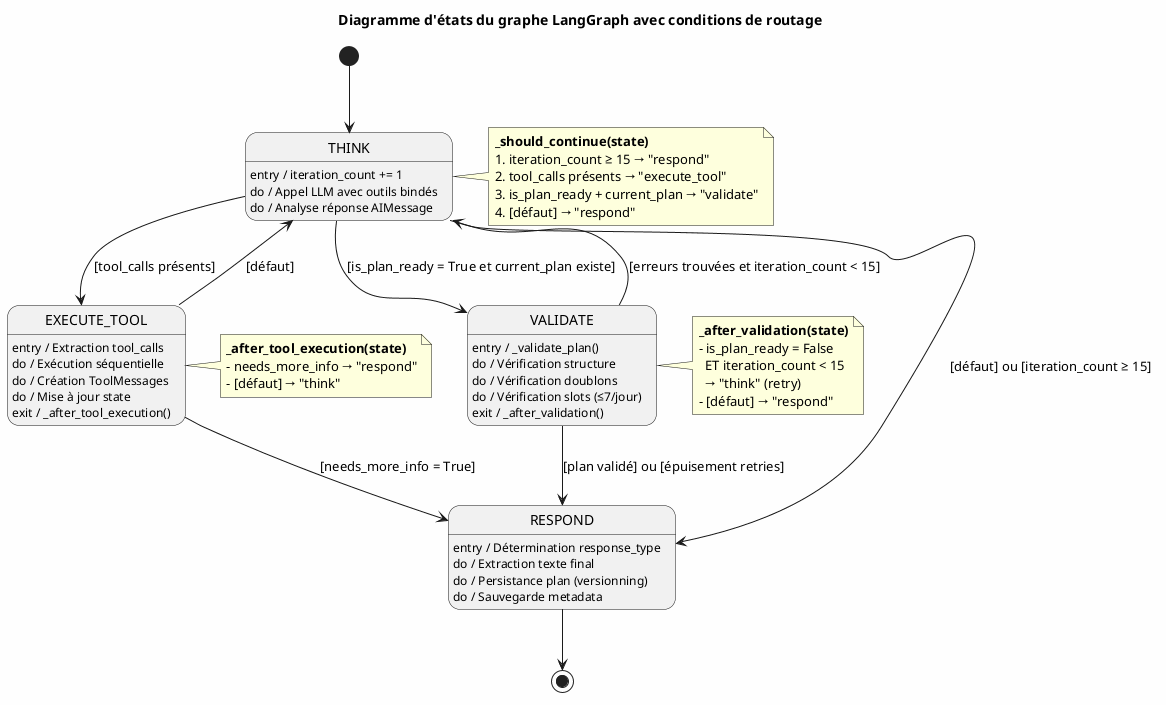
\includegraphics[width=\textwidth]{diagrams/fig_04_langgraph_routing.png}
    \caption{Diagramme d'états du graphe LangGraph avec conditions de routage}
    \label{fig:langgraph_routing}
\end{figure}


% ────────────────────────────────────────────────────────────────
\section{Le nœud THINK}
% ────────────────────────────────────────────────────────────────

\subsection{Construction du prompt système}

Le prompt système du module \texttt{personality.py} (122~lignes) définit l'identité de l'agent
Guidni comme un ami local chaleureux et expert du tourisme à Djerba, qui parle français, anglais
et arabe avec détection automatique de la langue de l'utilisateur. Le prompt interdit
explicitement à l'agent d'inventer des données~: il ne doit recommander que des lieux, activités
et hébergements effectivement récupérés par les outils de recherche. Les recommandations doivent
aller au-delà des clichés touristiques pour offrir des conseils authentiques d'initié.

Les règles comportementales encodées dans le prompt définissent les contraintes de planification
réaliste~: un maximum de 4 à 5~activités par jour, inclusion systématique de repas et de
périodes de repos, prise en compte des distances et de la logistique entre les lieux
(en utilisant l'outil \texttt{get\_distance}), variation des types d'activités pour éviter la
monotonie, et explication transparente du raisonnement derrière chaque recommandation. L'agent
doit réfléchir avant de répondre (principe ReAct), être honnête sur ses limitations, et
ne jamais forcer une recommandation si les données disponibles sont insuffisantes.

Le prompt contient également des règles cruciales de désambiguïsation des types d'entités~:
\texttt{activity} désigne une expérience payante (catégorie \og{}DO\fg{}), \texttt{stay} désigne
un hébergement uniquement (ne \emph{jamais} placer un hébergement dans un créneau d'activité
diurne), \texttt{restaurant}/\texttt{yummy} désigne un lieu de restauration (catégorie
\og{}EAT\fg{}), et \texttt{attraction} désigne un site touristique gratuit. Cette
désambiguïsation est essentielle car sans elle, le LLM peut confondre un hôtel avec une
attraction à visiter dans la journée.


\subsection{Injection du contexte dynamique}

Avant chaque appel au LLM, le nœud THINK construit un message de contexte à partir de l'état
courant. Si \texttt{user\_profile} existe, un résumé du profil est ajouté. Si
\texttt{current\_plan} existe, l'information \og{}version X avec N jours\fg{} est ajoutée. Si
\texttt{weather} existe, les prévisions météorologiques sont incluses. Si \texttt{rag\_context}
est non vide, les cinq premiers résultats sont formatés avec titre, type d'entité et score de
similarité. Ce contexte est injecté comme un \texttt{SystemMessage} distinct du prompt de
personnalité, permettant au LLM de voir clairement les données déjà collectées.

L'heuristique d'arrêt forcé constitue un mécanisme de sécurité critique~: si
\texttt{iteration\_count >= 2} et que \texttt{rag\_context} est non vide, un
\texttt{SystemMessage} final est injecté avec l'instruction~: \og{}IMPORTANT~: Vous avez déjà
suffisamment de données. Générez votre réponse FINALE maintenant. N'appelez PLUS d'outils de
recherche.\fg{} Cette heuristique empêche l'agent de rechercher indéfiniment lorsqu'il dispose
déjà d'un contexte suffisant, réduisant la latence et la consommation de tokens.

La normalisation du contenu spécifique à Gemini est gérée par les fonctions utilitaires
\texttt{\_get\_text\_content()} et \texttt{\_normalize\_content()}. Google Gemini retourne le
contenu des messages sous forme de liste de dictionnaires
(\texttt{[\{"type": "text", "text": "..."\}]}) au lieu d'une chaîne de caractères simple comme
Ollama et Groq. Ces fonctions détectent le format et extraient le texte de manière transparente,
assurant la compatibilité multi-fournisseurs sans modification du code des nœuds.


% ────────────────────────────────────────────────────────────────
\section{Les 18 outils LLM}
% ────────────────────────────────────────────────────────────────

\subsection{Vue d'ensemble et registre des outils}

Le décorateur \texttt{@tool} de LangChain transforme une fonction Python asynchrone en un outil
appelable par le LLM. La décoration analyse la signature de la fonction, sa docstring et ses
annotations de type pour générer automatiquement un schéma JSON décrivant le nom de l'outil, sa
description et les paramètres attendus. La méthode \texttt{bind\_tools()} de LangGraph attache
ensuite ces schémas au LLM pour que le modèle puisse émettre des appels d'outils structurés.

Le registre central défini dans \texttt{registry.py} exporte la fonction
\texttt{get\_all\_tools()} qui retourne les 18~outils dans un ordre fixe. Lors de l'exécution,
le nœud EXECUTE\_TOOL construit un dictionnaire de correspondance
\texttt{\{tool.name: tool\}} pour dispatcher les appels par nom. Les outils couvrent sept
domaines fonctionnels~: le profil utilisateur (1~outil), la recherche d'entités (5~outils),
la météo et la géolocalisation (3~outils), la disponibilité et le budget (3~outils), la
construction de plans (3~outils), la communication (1~outil) et la recherche sémantique
RAG (3~outils).

La gestion des erreurs suit un patron uniforme~: chaque outil encapsule ses requêtes de base
de données et ses appels API dans un bloc \texttt{try/except} et retourne un dictionnaire
\texttt{\{"error": "message"\}} plutôt que de lever une exception. Le LLM reçoit l'erreur
dans un \texttt{ToolMessage} et peut décider de réessayer avec des paramètres différents ou
d'informer l'utilisateur du problème. Ce patron garantit que le graphe LangGraph ne s'arrête
jamais brutalement à cause d'un outil défaillant.

\begin{table}[H]
    \centering
    \caption{Catalogue des 18 outils LLM}
    \label{tab:tools_catalog}
    \footnotesize
    \begin{tabular}{p{3.2cm} p{2.5cm} p{3.5cm} p{2cm} p{2.5cm}}
        \toprule
        \textbf{Outil} & \textbf{Module} & \textbf{Tables DB} & \textbf{API ext.} & \textbf{Retourne} \\
        \midrule
        get\_user\_profile & user\_tools & User, Reservation, Review, Wishlist, Preference & — & Profil dict \\[2pt]
        search\_activities & activity\_tools & Activity, Images & — & Liste activités \\[2pt]
        get\_activity\_details & activity\_tools & Activity, Images & — & Activité complète \\[2pt]
        enrich\_activity & activity\_tools & ActivityIntelligence & LLM & Enrichissement JSON \\[2pt]
        get\_weather & weather\_tools & — & Open-Meteo & Météo dict \\[2pt]
        get\_distance & geo\_tools & — & — (Haversine) & \{km, minutes\} \\[2pt]
        geocode\_address & geo\_tools & — & Nominatim & \{lat, lon\} \\[2pt]
        search\_stays & stay\_tools & Stay, Images & — & Liste hébergements \\[2pt]
        search\_restaurants & restaurant\_tools & Restaurant, Images, Hours & — & Liste restaurants \\[2pt]
        check\_availability & availability\_tools & Activity, Reservation & — & \{available, spots\} \\[2pt]
        estimate\_daily\_budget & budget\_tools & — & — & \{total, ventilation\} \\[2pt]
        estimate\_trip\_budget & budget\_tools & — & — & \{total, moy. jour\} \\[2pt]
        create\_plan\_structure & plan\_tools & Activity (valid.) & — & \{valid, plan\} \\[2pt]
        modify\_plan & plan\_tools & — & — & \{modified, plan\} \\[2pt]
        save\_plan\_tool & plan\_tools & GeneratedPlan & — & \{saved, id\} \\[2pt]
        ask\_user & communication & — & — & \{question, suggestions\} \\[2pt]
        rag\_search & rag\_tools & VectorStoreIndex & — & Résultats scorés \\[2pt]
        rag\_search\_for\_plan & rag\_tools & VectorStoreIndex & — & 4 listes thématiques \\[2pt]
        rag\_get\_similar & rag\_tools & VectorStoreIndex & — & Entités similaires \\
        \bottomrule
    \end{tabular}
\end{table}


\subsection{Outil rag\_search\_for\_plan~: quatre recherches parallèles}

L'outil \texttt{rag\_search\_for\_plan} est le plus complexe du registre car il adresse un
problème fondamental~: une requête RAG unique ne peut pas distinguer entre \og{}que faire\fg{}
(activités, attractions) et \og{}où manger\fg{} (restaurants) et \og{}où dormir\fg{}
(hébergements). Mélanger ces types dans une seule requête pollue les résultats car les vecteurs
d'embedding de \og{}hôtel 3 étoiles avec piscine\fg{} sont sémantiquement proches de
\og{}activité de natation\fg{}, produisant des recommandations incohérentes.

L'outil exécute quatre recherches parallèles avec des requêtes spécialisées~: la recherche
d'activités utilise la requête complète de l'utilisateur enrichie du thème de la journée~; la
recherche de restaurants utilise une requête alimentaire spécifique
(\og{}restaurant dining food cuisine local \{region\}\fg{}) indépendamment du thème du voyage,
car des thèmes comme \og{}journée aventure\fg{} ne correspondent pas aux vecteurs de description
des restaurants~; la recherche d'hébergements utilise la requête complète avec un filtre de
prix~; la recherche d'attractions utilise une requête patrimoniale (\og{}sightseeing landmark
museum heritage culture \{region\}\fg{}) pour trouver des sites gratuits.

La logique de dimensionnement adapte le nombre de résultats demandés à la durée du voyage.
Les formules utilisées sont~: $\min(\text{num\_days} \times 4, 20)$ pour les activités,
$\min(\text{num\_days} \times 2, 10)$ pour les restaurants, $\min(\text{num\_days}, 5)$ pour
les hébergements, et $\min(\text{num\_days} \times 2, 10)$ pour les attractions. Cette
adaptation empêche le sur-échantillonnage pour les voyages courts et le sous-échantillonnage
pour les voyages longs.

Le résultat retourné contient un champ \texttt{WARNING} proéminent~: \og{}stays are
ACCOMMODATION --- suggest as overnight stay ONLY, NEVER place them as daytime activities\fg{}.
Ce garde-fou textuel injecté dans la réponse de l'outil empêche le LLM de commettre l'erreur
de placer un hôtel dans un créneau d'activité diurne --- un problème récurrent lors des phases
de test qui corrompait les plans générés.


\subsection{Outil enrich\_activity~: cache d'intelligence IA}

L'outil \texttt{enrich\_activity} produit des métadonnées structurées que la base de données ne
contient pas nativement~: \texttt{noise\_level} (calme/modéré/bruyant), \texttt{ambiance}
(romantique/famille/aventure), \texttt{physical\_intensity} (faible/modérée/élevée),
\texttt{best\_time\_of\_day} (matin/après-midi/soir/indifférent), \texttt{ideal\_weather},
\texttt{ideal\_group\_type}, \texttt{age\_friendly}, \texttt{indoor\_outdoor}, \texttt{tags},
et un résumé en une phrase. Ces métadonnées permettent à l'agent de prendre des décisions de
planification plus intelligentes que le simple filtrage par catégorie.

Le mécanisme de cache repose sur la table \texttt{ActivityIntelligence}. Avant tout appel au LLM,
l'outil vérifie l'existence d'un enrichissement préexistant pour l'activité demandée. Si un
enrichissement est trouvé, il est retourné immédiatement sans appel LLM (coût nul, réponse
instantanée). Si aucun enrichissement n'existe, le LLM est appelé, la réponse JSON est analysée,
et le résultat est inséré dans la table via un \texttt{upsert}. Les appels ultérieurs pour la
même activité sont gratuits et instantanés.

En cas d'échec de l'appel LLM (erreur réseau, quota dépassé, JSON malformé), un enrichissement
de base est généré à partir du champ \texttt{categories} de l'activité. Par exemple, une
activité de catégorie \og{}water sports\fg{} reçoit automatiquement
\texttt{physical\_intensity="high"} et \texttt{indoor\_outdoor="outdoor"}. Ce mécanisme de
repli garantit que l'outil ne retourne jamais une erreur à l'agent, maintenant la fluidité
du cycle de raisonnement.
% ============================================================================
% CHAPITRE 4 — Part 2: 4.4–4.9 + Conclusion
% ============================================================================

% ────────────────────────────────────────────────────────────────
\section{Le nœud EXECUTE\_TOOL}
% ────────────────────────────────────────────────────────────────

Le nœud d'exécution des outils, défini dans \texttt{tool\_executor.py}, constitue le pont entre
les décisions du LLM et les systèmes de données. Il extrait tous les \texttt{tool\_calls} du
dernier \texttt{AIMessage}, construit un dictionnaire de correspondance
\texttt{\{name: tool\}} à partir du registre, et exécute chaque outil séquentiellement via
\texttt{await tool\_fn.ainvoke(tool\_args)}. Chaque résultat est encapsulé dans un
\texttt{ToolMessage} avec le contenu sérialisé en JSON compact et l'identifiant
\texttt{tool\_call\_id} pour la corrélation avec l'appel d'origine.

Les mises à jour critiques de l'état sont déclenchées par les résultats de certains outils.
Lorsque \texttt{create\_plan\_structure} retourne \texttt{result["valid"]=True}, l'exécuteur
met à jour \texttt{is\_plan\_ready=True} et \texttt{current\_plan=result["plan"]}, déclenchant
le routage vers VALIDATE. Lorsque \texttt{ask\_user} est invoqué,
\texttt{needs\_more\_info=True} et \texttt{questions} sont mis à jour, provoquant un routage
direct vers RESPOND. Les trois outils RAG (\texttt{rag\_search}, \texttt{rag\_search\_for\_plan},
\texttt{rag\_get\_similar}) mettent à jour le champ \texttt{rag\_context}~; dans le cas
spécifique de \texttt{rag\_search\_for\_plan}, les quatre sous-listes
(\texttt{activities\_for\_time\_slots}, \texttt{restaurants\_for\_meals},
\texttt{stays\_for\_overnight\_only}, \texttt{attractions\_for\_time\_slots}) sont aplaties en
une liste unifiée.

Pour chaque outil exécuté, une étape de réflexion (\textit{thinking step}) est créée avec une
description lisible par l'humain (par exemple \og{}$\checkmark$ search\_activities completed ---
Found 8 items\fg{}) et ajoutée à la liste accumulée \texttt{thinking\_steps}. En cas d'échec
d'un outil, un message d'erreur est créé (\og{}$\times$ tool\_name failed: message\fg{}) et
l'erreur est encapsulée dans un \texttt{ToolMessage} pour que le LLM puisse décider de la
marche à suivre. L'exécuteur effectue également une journalisation détaillée au niveau DEBUG,
incluant les arguments d'entrée complets et les résultats complets de chaque outil, facilitant
le débogage des chaînes de raisonnement complexes.

\begin{figure}[H]
    \centering
    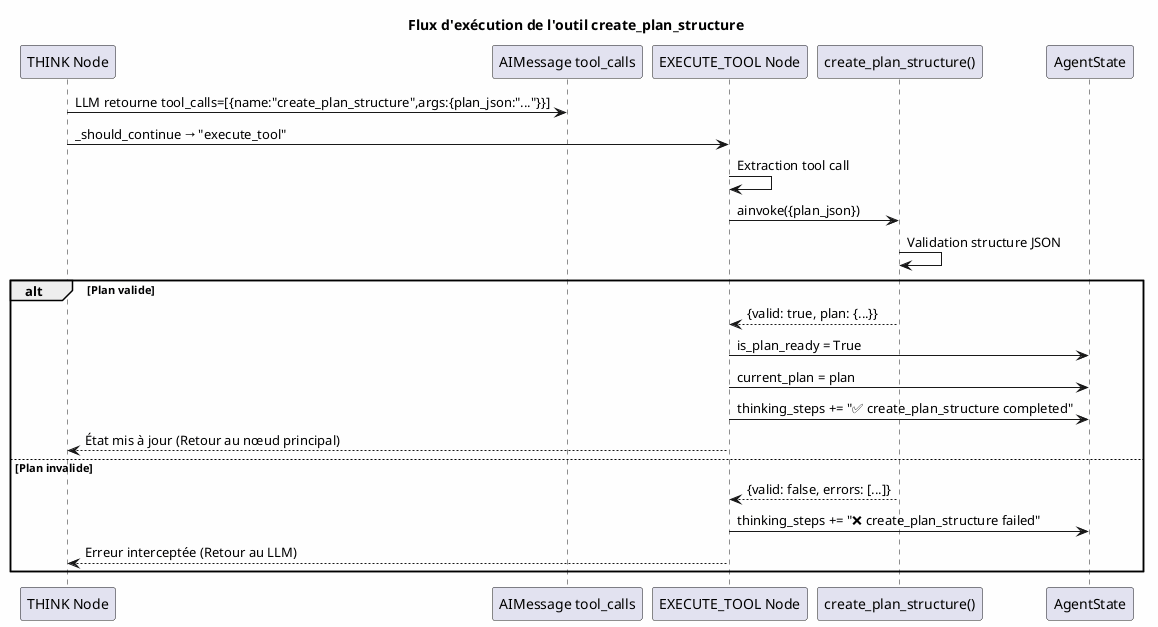
\includegraphics[width=\textwidth]{diagrams/fig_04_tool_execution_flow.png}
    \caption{Flux d'exécution de l'outil create\_plan\_structure}
    \label{fig:tool_exec_flow}
\end{figure}


% ────────────────────────────────────────────────────────────────
\section{Le nœud VALIDATE}
% ────────────────────────────────────────────────────────────────

Le nœud de validation, défini dans \texttt{validator.py}, implémente les garde-fous qui
empêchent la livraison de plans incohérents à l'utilisateur. La fonction
\texttt{\_validate\_plan()} vérifie quatre règles~: le plan doit contenir au moins un jour,
chaque jour doit comporter au moins un créneau, aucun jour ne doit dépasser 7~créneaux
(pour éviter les plannings irréalistes surchargeant la journée), et aucun
\texttt{activity\_id} ne doit apparaître plus d'une fois dans l'ensemble du plan (détection
des doublons).

Le mécanisme d'injection d'erreurs repose sur les \texttt{SystemMessage} de LangChain. Si des
erreurs de validation sont détectées, un message système est ajouté à la liste des messages
avec le contenu~: \og{}\texttt{[VALIDATION] Validation issues: Day 2 has duplicate activity
ID abc123; Day 3 has too many activities (9). Please fix these issues.}\fg{} Le champ
\texttt{is\_plan\_ready} est remis à \texttt{False}, et la fonction de routage
\texttt{\_after\_validation()} renvoie l'agent au nœud THINK. Le LLM lit le message d'erreur
et corrige le plan lors de son prochain appel d'outil.

Le choix d'injecter les erreurs comme \texttt{SystemMessage} plutôt que comme résultat d'outil
est un choix de conception délibéré. Les messages système sont traités avec une priorité élevée
par les LLMs (instruction de niveau système), tandis que les résultats d'outils peuvent être
enfouis dans un historique de messages long. Cette hiérarchie de priorité garantit que le LLM
prend les erreurs de validation au sérieux et les corrige effectivement.


% ────────────────────────────────────────────────────────────────
\section{Le nœud RESPOND et la persistance}
% ────────────────────────────────────────────────────────────────

Le nœud de réponse, défini dans \texttt{responder.py}, détermine le type de réponse selon
l'état courant~: si \texttt{needs\_more\_info} est \texttt{True} et \texttt{questions} est
non nul, le type est \texttt{"question"}~; si \texttt{is\_plan\_ready} est \texttt{True} et
\texttt{is\_modification} est \texttt{True}, le type est \texttt{"modification"}~; si
\texttt{is\_plan\_ready} est \texttt{True}, le type est \texttt{"plan"}~; sinon, le type est
\texttt{"text"} (réponse conversationnelle simple).

L'extraction du texte final parcourt la liste des messages en ordre inverse pour trouver le
dernier \texttt{AIMessage} avec un contenu non vide. Le contenu est normalisé via
\texttt{\_normalize\_content()} pour gérer le format liste-de-dictionnaires de Gemini.
Cette approche est nécessaire car dans un cycle multi-outils, plusieurs \texttt{ToolMessage}
peuvent suivre le dernier \texttt{AIMessage} contenant du texte, et il faut retrouver la
bonne source de texte.

La persistance des plans exploite le versionnement. Lorsque le type de réponse est
\texttt{"plan"} ou \texttt{"modification"}, la fonction \texttt{save\_plan()} est appelée.
Elle désactive d'abord tous les plans actifs existants pour cette conversation
(\texttt{UPDATE SET isActive=False}), puis détermine le numéro de version en comptant les
plans existants, et enfin insère une nouvelle ligne avec \texttt{isActive=True} et
\texttt{version=N+1}. Ce mécanisme de versionnement permet de récupérer les itérations
précédentes d'un plan si l'utilisateur souhaite revenir à une version antérieure.

Les métadonnées sauvegardées avec chaque message assistant comprennent la liste
\texttt{thinking\_steps}, la liste \texttt{tools\_used}, et le booléen \texttt{has\_plan}.
Ces métadonnées sont stockées dans la colonne JSON \texttt{metadata} de la table
\texttt{PlannerMessage}, permettant au frontend de reconstruire l'affichage des étapes de
réflexion à partir de l'historique de conversation sans nécessiter de nouveaux appels à l'agent.


% ────────────────────────────────────────────────────────────────
\section{Le pipeline RAG}
% ────────────────────────────────────────────────────────────────

L'architecture RAG a été présentée en détail au chapitre~2. Cette section se concentre sur les
aspects spécifiques de l'implémentation. Chaque type d'entité dispose d'une fonction dédiée de
construction de documents (\texttt{\_activity\_to\_document}, \texttt{\_stay\_to\_document},
\texttt{\_yummy\_to\_document}, \texttt{\_attraction\_to\_document}) qui convertit une instance
de modèle ORM en un \texttt{Document} LlamaIndex. Le document comprend un corps textuel riche
incluant tous les champs pertinents (titre, description, catégorie, région, prix, durée,
équipements) et un dictionnaire de métadonnées structurées contenant \texttt{entity\_type},
\texttt{entity\_id}, \texttt{title}, \texttt{category}, \texttt{region}, \texttt{city} et
\texttt{price}. Ces métadonnées sont utilisées pour le filtrage lors des requêtes.

La détection de changements par hachage optimise la réindexation incrémentale. Lorsqu'une
entité est modifiée en base de données, la fonction \texttt{upsert\_entity()} recalcule le
hash MD5 du texte du nouveau document et le compare au hash stocké dans le dictionnaire
\texttt{\_entity\_hashes}. Si le hash est identique, le recalcul coûteux des embeddings est
évité. Cette optimisation est particulièrement importante car le calcul d'un embedding par
le modèle BAAI/bge-m3 prend environ 200\,ms par document sur CPU.

La fonction \texttt{rag\_query()} implémente une stratégie de sur-échantillonnage~: le
récupérateur demande $\texttt{top\_k} \times 2$ résultats à l'index, puis filtre les résultats
par type d'entité, seuil de score et prix maximum, et enfin limite à \texttt{top\_k}. Ce
sur-échantillonnage compense le fait que les filtres de métadonnées dans LlamaIndex utilisent
une logique AND qui peut être trop restrictive pour les requêtes multi-types, éliminant des
résultats pertinents avant le post-filtrage applicatif.

\begin{figure}[H]
    \centering
    
\includegraphics[width=\textwidth]{diagrams/screen_04_rag_search_result.png}
    \caption{Exemple de résultats d'une recherche RAG avec scores de similarité}
    \label{fig:rag_results}
\end{figure}


% ────────────────────────────────────────────────────────────────
\section{Gestion de la mémoire et du contexte}
% ────────────────────────────────────────────────────────────────

\subsection{Chargement du contexte}

La fonction \texttt{load\_context()}, définie dans \texttt{conversation.py}, ouvre une session de
base de données et récupère la \texttt{PlannerConversation} avec ses 8~derniers
\texttt{PlannerMessage}. Chaque message est converti en son type LangChain correspondant~:
les messages de rôle \texttt{"user"} deviennent des \texttt{HumanMessage}, les messages
\texttt{"assistant"} des \texttt{AIMessage}, et les messages \texttt{"system"} des
\texttt{SystemMessage}. Le plan actif est ensuite récupéré via \texttt{get\_current\_plan()}.

Le choix d'une fenêtre de 8~messages résulte d'un compromis empirique. Charger moins de
messages risque de perdre un contexte pertinent (l'utilisateur a dit \og{}supprimez la journée
plage\fg{} mais cette journée a été mentionnée 12~messages plus tôt et n'est plus visible).
Charger plus de messages augmente la consommation de tokens et la latence de chaque appel LLM.
Huit messages représentent environ 2 à 4~tours de conversation, couvrant la plupart des
scénarios de modification de plans.

Si le champ \texttt{contextSummary} de la conversation est non nul (c'est-à-dire qu'un résumé
a été généré par le résumeur automatique), un \texttt{SystemMessage} est inséré en position~0
de la liste de messages contenant le résumé structuré. Cette injection donne au LLM une vue
compressée de l'historique complet de la conversation, même si seulement 8~messages bruts sont
chargés. Le résumé étant structuré en JSON (préférences confirmées, contraintes, modifications),
il est plus exploitable qu'une simple concaténation de messages anciens.


\subsection{Résumé automatique}

La fonction \texttt{summarize\_if\_needed()}, définie dans \texttt{summarizer.py}, vérifie deux
conditions avant de déclencher un résumé~: le nombre de messages doit dépasser
\texttt{CONVERSATION\_SUMMARY\_THRESHOLD} (15 par défaut), et au moins 10~nouveaux messages
doivent avoir été ajoutés depuis le dernier résumé. Si un résumé récent existe et que moins de
10~messages se sont accumulés, le résumé existant est conservé tel quel.

Le résumé est produit par un appel LLM dédié (\texttt{temperature=0.3}, \texttt{json\_mode=True})
avec pour instruction de générer un JSON structuré contenant~: \texttt{trip\_overview}
(description générale du voyage), \texttt{confirmed\_preferences} (préférences confirmées par
l'utilisateur), \texttt{confirmed\_constraints} (nombre de jours, budget, taille du groupe,
dates), \texttt{modifications\_made} (liste des modifications demandées),
\texttt{important\_notes} (notes importantes), et \texttt{message\_count} (nombre de messages
résumés). Ce format structuré est plus exploitable par l'agent qu'un résumé en texte libre.

En cas d'échec de l'appel LLM (réseau, quota, JSON invalide), un résumé de base est construit
à partir des métadonnées de la conversation (nombre de messages, outils utilisés, types de
réponses) sans nécessiter d'appel LLM. Ce mécanisme de repli garantit que la fonction ne
lève jamais d'exception et ne bloque jamais le flux principal de l'agent.


\subsection{Profil utilisateur}

L'outil \texttt{get\_user\_profile} collecte l'ensemble des données historiques de l'utilisateur
depuis la base de données~: les 30~dernières réservations d'activités, les avis publiés, les
éléments de la liste de souhaits, et les préférences déclarées. Il calcule la fréquence par
catégorie (\texttt{favorite\_categories} triées par nombre de réservations), les dépenses totales
et moyennes, la note moyenne donnée dans les avis, et la liste des activités en favoris. Ces
informations composent un dictionnaire de profil riche que le nœud THINK injecte dans le
contexte du LLM.

Ce profil influence directement la qualité des recommandations de l'agent~: le LLM sait avant
de générer un plan que cet utilisateur a réservé des sports nautiques 5~fois, dépense en
moyenne 80~TND par jour, possède 3~activités spa dans sa liste de souhaits, et attribue des
notes de 5~étoiles aux tours culturels. Cette connaissance du profil permet des recommandations
véritablement personnalisées sans recours au moteur LinUCB --- l'agent adapte son raisonnement
à l'historique comportemental de chaque utilisateur.


% ────────────────────────────────────────────────────────────────
\section{Pipeline rapide de génération de plans}
% ────────────────────────────────────────────────────────────────

Le pipeline rapide existe en complément de la boucle agentique complète pour répondre à un
besoin spécifique~: la boucle complète de l'agent nécessite 15 à 40~secondes (appels LLM
multiples, exécutions d'outils, boucle de validation), ce qui est acceptable pour une
conversation exploratoire mais excessif lorsque l'utilisateur fournit toutes les informations
nécessaires en un seul message structuré (dates, taille du groupe, budget, préférences).

La détection automatique est assurée par la fonction \texttt{parse\_chat\_to\_plan\_request()},
qui analyse le message de l'utilisateur à la recherche d'informations structurées~: dates ou
durée en jours, mention de budget, composition du groupe (famille, couple, solo). Si ces
éléments sont détectés, un objet \texttt{UserPreferences} est construit et le pipeline rapide
est invoqué à la place de la boucle agentique, sans que l'utilisateur ne perçoive la différence
dans l'interface.

Le pipeline s'exécute en trois phases. La \textbf{phase~1} collecte toutes les données en
parallèle via \texttt{asyncio.gather()}~: recherche RAG thématique
(\texttt{rag\_search\_for\_plan}), prévisions météorologiques (\texttt{get\_weather}), calcul
des distances entre les lieux, et estimation du budget total (\texttt{estimate\_trip\_budget}).
La \textbf{phase~2} pré-traite les contraintes~: filtrage par budget, suppression des activités
incompatibles avec la météo, regroupement par proximité géographique. La \textbf{phase~3}
effectue un unique appel LLM avec toutes les données pré-chargées en contexte pour produire
le plan JSON final.

Le compromis est explicite~: le pipeline rapide sacrifie la profondeur conversationnelle et la
boucle de validation de l'agent complet au profit de la vitesse (5 à 10~secondes au lieu de
15 à 40). Il est approprié pour les utilisateurs expérimentés qui fournissent des informations
complètes dès le départ, tandis que l'agent complet est préférable pour les conversations
exploratoires où les besoins de l'utilisateur se précisent progressivement.

\begin{figure}[H]
    \centering
    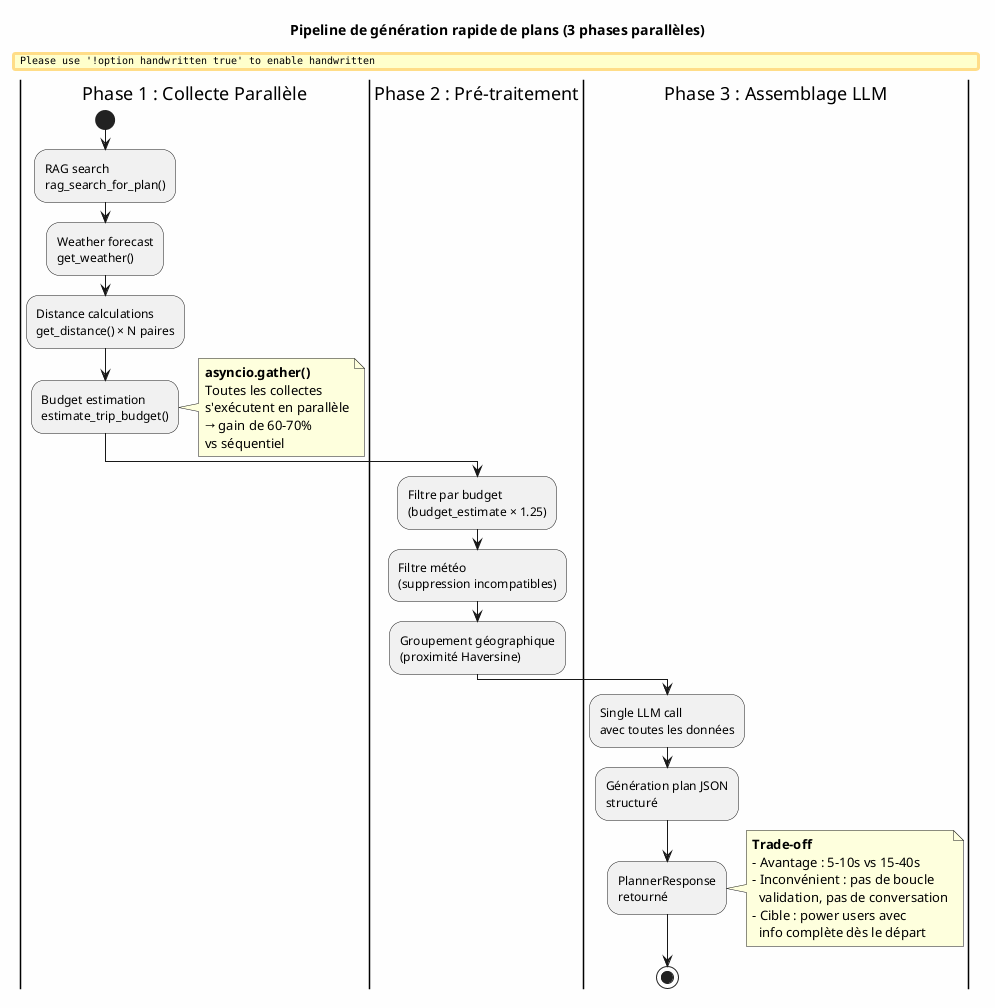
\includegraphics[width=\textwidth]{diagrams/fig_04_fast_pipeline.png}
    \caption{Pipeline de génération rapide de plans (3 phases parallèles)}
    \label{fig:fast_pipeline}
\end{figure}

\begin{figure}[H]
    \centering
    
\includegraphics[width=\textwidth]{diagrams/screen_04_chat_plan_output.png}
    \caption{Exemple de plan de voyage généré par l'agent Guidni}
    \label{fig:chat_output}
\end{figure}


% ────────────────────────────────────────────────────────────────
\section*{Conclusion du chapitre}
\addcontentsline{toc}{section}{Conclusion du chapitre}

Ce chapitre a présenté l'implémentation complète de l'agent planificateur IA du système Guidni.
La machine à états LangGraph avec ses quatre nœuds (THINK, EXECUTE\_TOOL, VALIDATE, RESPOND)
et ses trois fonctions de routage conditionnel a été détaillée, incluant les mécanismes de
sécurité (arrêt forcé à 15~itérations, heuristique de force-stop à 2~itérations avec contexte
RAG). Les 18~outils ont été catalogués et les plus complexes décrits en profondeur~:
\texttt{rag\_search\_for\_plan} avec ses quatre recherches parallèles et son garde-fou de
désambiguïsation des types d'entités, et \texttt{enrich\_activity} avec son cache
d'intelligence IA. Le pipeline RAG, le système de mémoire conversationnelle (fenêtre de
8~messages, résumé automatique au seuil de 15~messages, profil utilisateur), et le pipeline
rapide de génération de plans en trois phases ont complété la présentation.

Le chapitre suivant présente l'implémentation du second sous-système~: le moteur de
recommandation Hybrid LinUCB, avec son ingénierie des caractéristiques, son cycle
d'apprentissage en ligne, et son pipeline de classement en neuf étapes.
